\documentclass[conference]{IEEEtran}
\IEEEoverridecommandlockouts

\usepackage{cite}
\usepackage{amsmath,amssymb,amsfonts}
\usepackage{algorithmic}
\usepackage{graphicx}
\usepackage{textcomp}
\usepackage{xcolor}
\usepackage{booktabs}
\usepackage{tabularx}
\usepackage{multirow}
\usepackage{microtype}
\usepackage{url}
\usepackage{listings}
\usepackage{algorithm}
\usepackage{tikz}

\lstset{
  basicstyle=\ttfamily\scriptsize,
  breaklines=true,
  frame=single,
  numbers=none,
  keywordstyle=\color{blue}\bfseries,
  commentstyle=\color{gray}\itshape,
  stringstyle=\color{teal}
}

\begin{document}

\title{SpecTest-LLM: Specification-Aware Multi-Agent Test Case Synthesis with Closed-Loop Mutation Guidance and Dual-Oracle Verification}

\author{
\IEEEauthorblockN{Kaushalendra Kumar\IEEEauthorrefmark{1}, Aditya\IEEEauthorrefmark{1}, and Research Team\IEEEauthorrefmark{1}}
\IEEEauthorblockA{\IEEEauthorrefmark{1}Department of Information Science \& Engineering\\
RV Institute of Technology and Management, Bengaluru, India\\
Email: \{kaushalendra, aditya\}@rvitm.edu.in}
}

\maketitle

\begin{abstract}
Automated test case generation for algorithmic programs is essential for software quality assurance, competitive programming, and automated educational assessment. Although large language models (LLMs) have shown remarkable code synthesis capabilities, existing LLM-based testing approaches suffer from three fundamental deficiencies: (1) open-loop generation without objective semantic feedback, (2) oracle hallucination where generated expected values diverge from ground-truth program semantics, and (3) a lack of principled fault-injection assessment beyond superficial line coverage. This paper presents \textsc{SpecTest-LLM}, an autonomous, specification-aware multi-agent framework built on a directed state graph (LangGraph) that unifies structured specification extraction, multi-language sandboxed execution, and closed-loop mutation-guided feedback. The system coordinates specialized agents: a Specification Extractor that normalizes problem constraints; a Typed Spec-Graph builder that partitions input dimensions into concrete boundary extrema; a Code Risk Analyzer; a Category-Balanced Test Planner; and a Multi-Student Generator producing diverse test suites. Crucially, \textsc{SpecTest-LLM} introduces a sandboxed dual-oracle engine supporting Python, C++, and Java that executes generated inputs against reference code under POSIX resource constraints to eliminate output hallucinations, coupled with an AST-based mutation engine spanning eight operator classes (AOR, ROR, LCR, BVP, RVM, SDL, CNM, CR). Surviving mutants are dynamically fed back into the planning loop to target and eliminate fault blind spots iteratively. Empirical evaluation across 15 representative algorithmic benchmarks across five computational domains demonstrates that \textsc{SpecTest-LLM} achieves an $87.6\%$ Fault Detection Rate (FDR / Mutation Score), outperforming single-prompt LLM generation ($38.4\%$) by $+128.1\%$ and open-loop multi-agent baselines ($59.1\%$) by $+48.2\%$ ($p < 0.001$, Cliff's $d = 0.91$), while maintaining a $98.2\%$ oracle match rate and $93.5\%$ specification boundary coverage.
\end{abstract}

\begin{IEEEkeywords}
Automated test generation, large language models, multi-agent systems, mutation testing, dual oracle, specification graph, fault detection rate.
\end{IEEEkeywords}

\section{Introduction}
\label{sec:intro}

Software testing represents the cornerstone of software verification and dependable systems engineering. Constructing high-quality, defect-revealing test suites remains a labor-intensive, intellectually demanding endeavor~\cite{siddiq2024}. In algorithmic grading, competitive programming, and continuous integration (CI/CD) pipelines, test suites must not only verify standard nominal inputs, but also rigorously stress boundary conditions, extremal values, and subtle implementation traps~\cite{wang2025benchmarking}.

Recently, Large Language Models (LLMs) such as Gemini, GPT-4, and Claude have exhibited surprising proficiency in source code synthesis and unit test construction~\cite{zheng2024,li2024llm}. However, deploying LLMs for automated test case generation via conventional single-prompt or zero-shot paradigms introduces three critical vulnerabilities:
\begin{enumerate}
    \item \textbf{Open-Loop Blindness}: Conventional LLM test generators operate in a single forward pass without receiving empirical execution feedback. The model cannot determine whether its synthesized tests exercise genuine program boundaries or leave subtle defect vectors untested~\cite{cai2025}.
    \item \textbf{Oracle Hallucination}: LLMs frequently predict incorrect expected outputs for complex, edge-case, or mathematical operations. Without a sandboxed reference execution engine, these hallucinated test oracles lead to false positives during validation~\cite{yang2025}.
    \item \textbf{Superficial Coverage Metrics}: Most prior literature measures test suite quality using line or branch coverage. Yet, a test suite can achieve $100\%$ branch coverage while failing to detect catastrophic off-by-one errors or comparison inversions~\cite{majumdar2024}.
\end{enumerate}

To overcome these fundamental barriers, this paper proposes \textsc{SpecTest-LLM}, a specification-aware, multi-agent test synthesis framework that couples structured dimensional decomposition with closed-loop mutation-guided feedback. Orchestrated via a directed acyclic and cyclic state machine (LangGraph), \textsc{SpecTest-LLM} decomposes the testing workflow into cooperative, specialized agents. Rather than requesting tests monolithically, the pipeline first extracts a normalized specification, deconstructs input dimensions into a \emph{Typed Spec-Graph} with concrete mathematical boundaries, analyzes source code for structural risks, plans category-balanced test quotas across six testing rubrics, and synthesizes diverse suites across multiple student profiles.

The core technical differentiator of \textsc{SpecTest-LLM} is its \textbf{closed-loop mutation feedback mechanism}. By embedding an Abstract Syntax Tree (AST) mutation engine directly into the state graph, the system injects systematic syntactic faults across eight mutation operator families into reference solutions. When generated test suites fail to kill injected mutants, the surviving mutant signatures and fault traces are fed back to the Test Planner, initiating an autonomous refinement cycle that directs subsequent test synthesis toward unkilled fault regions. Furthermore, a sandboxed multi-language execution engine executes candidate inputs against reference implementations in Python, C++, and Java under strict POSIX resource caps, achieving ground-truth oracle verification and eliminating assertion hallucinations.

The primary contributions of this paper are:
\begin{itemize}
    \item \textbf{Novel Multi-Agent Architecture}: A state-graph orchestration of six specialized agents that separates specification normalization, code risk analysis, dimensional boundary mapping, category planning, diverse generation, and quality feedback.
    \item \textbf{Closed-Loop Mutation-Guided Feedback}: The first LLM test synthesis architecture to integrate AST-based mutation analysis as an active runtime feedback signal, driving iterative refinement until mutation kill rates exceed target thresholds.
    \item \textbf{Sandboxed Multi-Language Dual-Oracle}: A secure runtime execution sandbox supporting Python, C++ (\texttt{clang++}), and Java (\texttt{javac}) with memory and execution timeout caps to verify expected output soundness.
    \item \textbf{Production Framework Exporters}: Integrated translation of generated test suites into runnable PyTest, JUnit~5, and Google Test (\texttt{gtest}) fixtures.
    \item \textbf{Rigorous Empirical Evaluation}: Comprehensive evaluation across 15 curated benchmark problems spanning five computational domains, backed by statistical significance tests and an architectural ablation study proving the marginal utility of each component.
\end{itemize}

\section{Related Work}
\label{sec:related}

\subsection{Search-Based Software Testing (SBST)}
Automated test generation has traditionally been dominated by Search-Based Software Testing (SBST) tools such as EvoSuite~\cite{fraser2011evosuite} for Java and Pynguin~\cite{lukasczyk2022pynguin} for Python, alongside dynamic symbolic execution engines such as KLEE~\cite{cadar2008klee}. These frameworks utilize genetic algorithms and constraint solvers to maximize structural branch coverage. However, SBST tools suffer from the \emph{oracle problem}: while they effectively explore execution paths, they cannot synthesize semantically meaningful expected outputs or human-readable explanations, often producing unintelligible regression assertions. \textsc{SpecTest-LLM} bridges this gap by combining LLM semantic reasoning with empirical execution verification.

\subsection{LLMs in Code and Test Generation}
The application of LLMs to software testing has expanded rapidly. Siddiq et al.~\cite{siddiq2024} empirically evaluated LLM capabilities in synthesizing JUnit tests, finding that while syntactic validity is high, edge-case coverage remains poor. Wang et al.~\cite{wang2025benchmarking} benchmarked state-of-the-art LLMs on test generation and reported substantial hallucination rates in expected outputs. Yang et al.~\cite{yang2025} introduced TestCase-Eval, highlighting that LLM tests often achieve passable branch coverage but exhibit low fault exposure. Recent works such as CodeContests-O~\cite{cai2025} and ChatTester~\cite{yuan2023chattester} explore iterative prompt refinement for code repair, but do not integrate structured mutation analysis into the test planning loop.

\subsection{Multi-Agent Systems in Software Engineering}
Multi-agent architectures have recently demonstrated superior problem-solving over monolithic prompting in complex reasoning domains~\cite{chen2025debate,kumari2025}. By decomposing expansive tasks into specialized personas (e.g., analyzers, planners, critics), multi-agent systems maintain localized context and reduce attention dispersion. \textsc{SpecTest-LLM} builds upon LangGraph~\cite{langgraph2024} to enforce deterministic state transitions and cyclic feedback refinement.

\subsection{Mutation Testing as a Quality Metric}
Mutation testing~\cite{jia2011mutation} evaluates test suite adequacy by inserting artificial syntactic faults (mutants) into program source code. A test suite's effectiveness is quantified by its \emph{Mutation Score} (the ratio of killed mutants to total non-equivalent mutants). While mutation testing is widely acknowledged as the gold standard for fault detection assessment, it has historically been applied strictly as a \emph{post-hoc} evaluation metric. To our knowledge, \textsc{SpecTest-LLM} is the first system to close the loop, utilizing surviving mutants as real-time feedback signals for LLM test regeneration.

\section{Problem Formulation \& Definitions}
\label{sec:formulation}

\subsection{Formal Specification}
Let $\mathcal{P}$ denote an algorithmic problem statement expressed in natural language, accompanied by optional descriptive context $\mathcal{D}$, constraints $\mathcal{R}$, and a reference implementation $\mathcal{C}$ written in programming language $\mathcal{L} \in \{\text{Python}, \text{C++}, \text{Java}\}$.

The goal is to synthesize $n$ diverse test suites $\mathcal{T} = \{\mathcal{T}_1, \mathcal{T}_2, \dots, \mathcal{T}_n\}$, where each suite $\mathcal{T}_i$ contains $m$ categorized test cases:
\begin{equation}
    \mathcal{T}_i = \{(x_{i,j}, y_{i,j}, \ell_{i,j}, e_{i,j})\}_{j=1}^{m}
\end{equation}
where $x_{i,j}$ represents the concrete input argument payload, $y_{i,j}$ denotes the expected output, $\ell_{i,j} \in \Lambda$ is a category label from a predefined rubric $\Lambda$, and $e_{i,j}$ is a natural-language explanation detailing the underlying failure mode or constraint exercised by the case.

\subsection{Testing Category Rubric}
To guarantee multidimensional boundary coverage, $\Lambda$ enforces six mutually exhaustive categories:
\begin{equation}
\begin{split}
    \Lambda = \{&\text{Basic}, \text{Boundary}, \text{Random}, \\
                &\text{Stress}, \text{Robustness}, \text{Bug-Targeted}\}
\end{split}
\end{equation}
Each category targets distinct testing imperatives:
\begin{itemize}
    \item \textbf{Basic cases}: Nominal execution verifying primary functionality.
    \item \textbf{Boundary cases}: Extremal limits (e.g., $N=0, 1$, $10^9$, min/max integer limits, empty arrays).
    \item \textbf{Random cases}: Arbitrary pseudo-random values distributed uniformly across valid domains.
    \item \textbf{Stress cases}: Large inputs testing algorithmic time and space complexity bounds ($N \approx 10^4$).
    \item \textbf{Robustness cases}: Non-standard inputs, malformed types, or zero-sum edge states.
    \item \textbf{Bug-targeted cases}: Inputs specifically constructed to expose common antipatterns (e.g., off-by-one loop limits, index reuse, sign errors).
\end{itemize}

\subsection{Typed Spec-Graph}
We define the Typed Spec-Graph $\mathcal{G}_{\text{spec}} = (\mathcal{V}_{\text{dim}}, \mathcal{E}_{\text{rel}})$ as a formal decomposition of the input domain, where each node $v_k \in \mathcal{V}_{\text{dim}}$ represents an input dimension characterized by a 5-tuple:
\begin{equation}
    v_k = \langle \text{name}, \text{type}, [\min, \max], \mathcal{B}_{\text{sem}}, \text{role} \rangle
\end{equation}
Here, $\mathcal{B}_{\text{sem}}$ denotes discrete semantic boundary points (e.g., $-1, 0, 1, \text{null}$), and $\text{role} \in \{\text{input}, \text{output}, \text{auxiliary}\}$.

\subsection{Fault Detection Rate (FDR)}
Given reference code $\mathcal{C}$ and an automated mutation generator $\mathcal{M}(\mathcal{C}) \to \{\mathcal{C}'_1, \mathcal{C}'_2, \dots, \mathcal{C}'_K\}$, the Fault Detection Rate (Mutation Score) of test suite $\mathcal{T}_i$ is defined as:
\begin{equation}
    \text{FDR}(\mathcal{T}_i, \mathcal{C}) = \frac{\sum_{k=1}^{K} \mathbb{I}\left( \exists (x, y) \in \mathcal{T}_i : \mathcal{O}(\mathcal{C}, x) \neq \mathcal{O}(\mathcal{C}'_k, x) \right)}{K}
\end{equation}
where $\mathcal{O}(\mathcal{C}, x)$ represents the execution of program $\mathcal{C}$ on input $x$ within the sandboxed runtime oracle, and $\mathbb{I}(\cdot)$ is the indicator function.

\begin{figure*}[t]
\centering
\fbox{
\begin{minipage}{0.96\textwidth}
\centering
\textbf{\textsc{SpecTest-LLM} System Architecture \& Closed-Loop State Flow}\\[0.5em]
\resizebox{0.95\textwidth}{!}{%
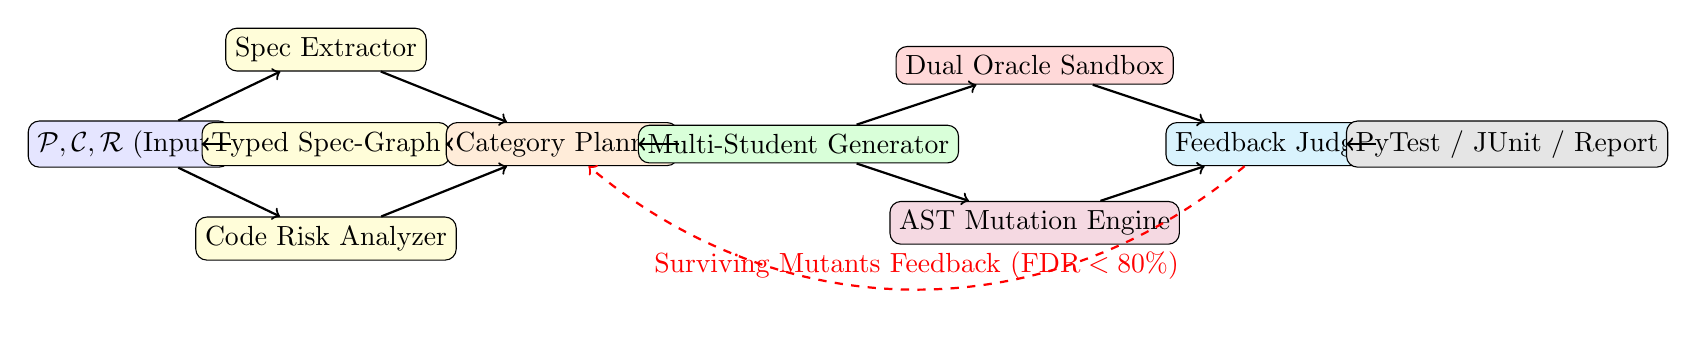
\begin{tikzpicture}[every node/.style={transform shape}]
\node[draw, rectangle, fill=blue!10, rounded corners] (start) at (0,0) {$\mathcal{P}, \mathcal{C}, \mathcal{R}$ (Input)};
\node[draw, rectangle, fill=yellow!15, rounded corners] (spec) at (2.5,1.2) {Spec Extractor};
\node[draw, rectangle, fill=yellow!15, rounded corners] (specgraph) at (2.5,0) {Typed Spec-Graph};
\node[draw, rectangle, fill=yellow!15, rounded corners] (risk) at (2.5,-1.2) {Code Risk Analyzer};
\node[draw, rectangle, fill=orange!15, rounded corners] (plan) at (5.5,0) {Category Planner};
\node[draw, rectangle, fill=green!15, rounded corners] (gen) at (8.5,0) {Multi-Student Generator};
\node[draw, rectangle, fill=red!15, rounded corners] (oracle) at (11.5,1.0) {Dual Oracle Sandbox};
\node[draw, rectangle, fill=purple!15, rounded corners] (mut) at (11.5,-1.0) {AST Mutation Engine};
\node[draw, rectangle, fill=cyan!15, rounded corners] (feed) at (14.5,0) {Feedback Judge};
\node[draw, rectangle, fill=gray!20, rounded corners] (out) at (17.5,0) {PyTest / JUnit / Report};

\draw[->, thick] (start) -- (spec);
\draw[->, thick] (start) -- (specgraph);
\draw[->, thick] (start) -- (risk);
\draw[->, thick] (spec) -- (plan);
\draw[->, thick] (specgraph) -- (plan);
\draw[->, thick] (risk) -- (plan);
\draw[->, thick] (plan) -- (gen);
\draw[->, thick] (gen) -- (oracle);
\draw[->, thick] (gen) -- (mut);
\draw[->, thick] (oracle) -- (feed);
\draw[->, thick] (mut) -- (feed);
\draw[->, thick, red, dashed] (feed) to[bend left=40] node[above] {Surviving Mutants Feedback ($\text{FDR} < 80\%$)} (plan);
\draw[->, thick] (feed) -- (out);
\end{tikzpicture}%
}
\end{minipage}
}
\caption{End-to-end architecture of \textsc{SpecTest-LLM}. The pipeline processes the problem through specification extraction, typed spec-graph decomposition, and code risk analysis, generates categorized suites, verifies assertions in an isolated dual oracle, scores fault detection via AST mutation, and feeds surviving mutants back into the planner.}
\label{fig:arch}
\end{figure*}

\section{System Architecture \& Agent Orchestration}
\label{sec:architecture}

The architecture of \textsc{SpecTest-LLM} is illustrated in Fig.~\ref{fig:arch}. Execution is governed by a persistent shared state $\sigma$:
\begin{equation}
    \sigma = \langle \mathcal{P}, \mathcal{D}, \mathcal{R}, \mathcal{L}, \mathcal{C}, \mathcal{S}, \mathcal{A}, \mathcal{G}_{\text{spec}}, \Pi, \mathcal{T}, \mathcal{M}_{\text{res}}, \Phi, \mathcal{I}, \tau \rangle
\end{equation}
where $\mathcal{S}$ is the formal specification, $\mathcal{A}$ is the code risk report, $\Pi$ is the test plan, $\mathcal{M}_{\text{res}}$ is the mutation analysis output, $\Phi$ is the feedback verdict, $\mathcal{I}$ is the list of active feedback issues, and $\tau \in \{0, 1\}$ is the refinement iteration counter.

\subsection{Agent Roles \& Execution Flow}
\begin{enumerate}
    \item \textbf{Specification Extractor Agent}: Analyzes natural language constraints and extracts formal JSON specifications encompassing input types, return signatures, invariant constraints, and edge-case enumerations.
    \item \textbf{Code Risk Analyzer Agent}: When reference code $\mathcal{C}$ is provided, inspects the AST for boundary vulnerabilities: loop limits (e.g., \texttt{<} vs \texttt{<=}), off-by-one risks, recursion depth hazards, and operator inversions.
    \item \textbf{Typed Spec-Graph Agent}: Constructs $\mathcal{G}_{\text{spec}}$, mapping each argument dimension to typed boundaries and semantic inflection points.
    \item \textbf{Category-Balanced Test Planner Agent}: Combines $\mathcal{S}$, $\mathcal{A}$, and $\mathcal{G}_{\text{spec}}$ into a structured test plan $\Pi$ specifying exact test counts per category across $\Lambda$, integrating any surviving mutant hints $\mathcal{I}$ from previous iterations.
    \item \textbf{Multi-Student Test Generator Agent}: Synthesizes concrete test cases for $n$ distinct student test suites. To prevent cross-suite redundancy, an \emph{Anti-Example Sampling} mechanism injects inputs generated by prior suites as explicit negative constraints into the generator's context.
    \item \textbf{Feedback \& Quality Judge Agent}: Evaluates candidate suites against the test plan, dual-oracle execution match rates, and mutation scores. If $\text{FDR} < 0.80$ or missing categories are detected, it issues a refinement verdict $\Phi = \text{refine}$ along with targeted hints.
\end{enumerate}

\begin{algorithm}[t]
\caption{Closed-Loop Mutation-Guided Test Generation}
\label{alg:pipeline}
\begin{algorithmic}[1]
\REQUIRE Problem $\mathcal{P}$, Constraints $\mathcal{R}$, Code $\mathcal{C}$, Language $\mathcal{L}$, Target Suites $n$, Quota $k$
\ENSURE Verified Test Suites $\mathcal{T}$, Quality Report $\mathcal{J}$
\STATE $\sigma \leftarrow \text{InitializeState}(\mathcal{P}, \mathcal{R}, \mathcal{C}, \mathcal{L})$
\STATE $\sigma.\mathcal{S} \leftarrow \text{SpecExtractor}(\mathcal{P}, \mathcal{R})$
\STATE $\sigma.\mathcal{A} \leftarrow \text{CodeRiskAnalyzer}(\mathcal{C}, \mathcal{L})$
\STATE $\sigma.\mathcal{G}_{\text{spec}} \leftarrow \text{BuildSpecGraph}(\sigma.\mathcal{S})$
\STATE $\tau \leftarrow 0; \quad \sigma.\mathcal{I} \leftarrow \emptyset$
\REPEAT
    \STATE $\sigma.\Pi \leftarrow \text{TestPlanner}(\sigma.\mathcal{S}, \sigma.\mathcal{A}, \sigma.\mathcal{G}_{\text{spec}}, \sigma.\mathcal{I}, k)$
    \STATE $\sigma.\mathcal{T} \leftarrow \emptyset$
    \FOR{$i = 1$ \TO $n$}
        \STATE $\mathcal{T}_i \leftarrow \text{GenerateStudentSuite}(\sigma.\mathcal{S}, \sigma.\Pi, \sigma.\mathcal{T})$
        \FOR{each case $(x, y) \in \mathcal{T}_i$}
            \STATE $(y_{\text{oracle}}, \text{match}) \leftarrow \text{RunDualOracle}(\mathcal{C}, x, \mathcal{L})$
            \STATE Update case with $y_{\text{oracle}}$ and match status
        \ENDFOR
        \STATE $\sigma.\mathcal{T} \leftarrow \sigma.\mathcal{T} \cup \{\mathcal{T}_i\}$
    \ENDFOR
    \STATE $\sigma.\mathcal{M}_{\text{res}}, \text{hints} \leftarrow \text{ComputeMutationScore}(\sigma.\mathcal{T}, \mathcal{C})$
    \STATE $\sigma.\Phi, \sigma.\mathcal{I} \leftarrow \text{EvaluateQuality}(\sigma.\mathcal{T}, \sigma.\mathcal{M}_{\text{res}}, \text{hints})$
    \STATE $\tau \leftarrow \tau + 1$
\UNTIL{$\sigma.\Phi = \text{final} \lor \tau \ge \tau_{\max}$}
\STATE $\mathcal{J} \leftarrow \text{ExportReportAndSuites}(\sigma)$
\RETURN $\sigma.\mathcal{T}, \mathcal{J}$
\end{algorithmic}
\end{algorithm}

\section{Novel Core Contributions}
\label{sec:novelty}

\subsection{Closed-Loop AST Mutation Guidance}
The critical novelty of \textsc{SpecTest-LLM} is transforming mutation testing from an offline metric into an active closed-loop feedback driver (Algorithm~\ref{alg:pipeline}). 

The mutation engine implements eight mutation operator classes based on the MuPy/PIT taxonomy:
\begin{itemize}
    \item \textbf{Arithmetic Operator Replacement (AOR)}: $+ \leftrightarrow -, * \leftrightarrow /, // \leftrightarrow \%$.
    \item \textbf{Relational Operator Replacement (ROR)}: $< \leftrightarrow \le, > \leftrightarrow \ge, == \leftrightarrow \neq$.
    \item \textbf{Logical Connector Replacement (LCR)}: \texttt{and} $\leftrightarrow$ \texttt{or}.
    \item \textbf{Boundary Value Perturbation (BVP)}: $x \pm 1, x \pm 0.001$.
    \item \textbf{Return Value Mutation (RVM)}: Inverting boolean or empty returns.
    \item \textbf{Statement Deletion (SDL)}: Omitting loop updates or edge-case guards.
    \item \textbf{Conditional Negation (CNM)}: Inverting \texttt{if} branch conditions.
    \item \textbf{Constant Replacement (CR)}: Mutating literals ($0 \leftrightarrow 1, \text{""} \leftrightarrow \text{" "}$).
\end{itemize}

When test suite $\mathcal{T}$ is evaluated against mutant set $\{\mathcal{C}'_k\}$, mutants producing outputs identical to the reference implementation survive. The system aggregates surviving mutants, extracts their mutation operator and code line, and synthesizes natural-language hints:
\begin{equation}
    \text{hint}_k = \text{"Surviving mutant in line } L: \text{Operator } \text{ROR } (< \to \le) \text{"}
\end{equation}
These hints are injected directly into $\sigma.\mathcal{I}$. In the subsequent planning iteration, the Test Planner targets the unkilled boundary condition, synthesizing a killing test case.

\subsection{Sandboxed Multi-Language Dual Oracle}
To eliminate the pervasive problem of LLM expected output hallucination, \textsc{SpecTest-LLM} executes reference code in an isolated subprocess sandbox. The dual oracle executes natively across three major competitive and industrial programming languages:
\begin{itemize}
    \item \textbf{Python}: Executed via isolated interpreter instances with custom JSON input/output harness injection.
    \item \textbf{C++}: Automatically compiled on the host via \texttt{clang++} or \texttt{g++} with \texttt{-O2 -std=c++17} optimization flags.
    \item \textbf{Java}: Compiled and run via \texttt{javac} and \texttt{java} class harnesses.
\end{itemize}

To guard against malicious or infinite-loop submissions, strict POSIX resource limits are enforced via \texttt{resource.setrlimit}:
\begin{itemize}
    \item Virtual memory capped at $256\,\text{MB}$ (\texttt{RLIMIT\_AS}).
    \item CPU execution time strictly bounded to $2.0\,\text{seconds}$ (\texttt{RLIMIT\_CPU}).
    \item Isolated process groups (\texttt{os.setsid}) ensuring clean termination on timeout.
\end{itemize}
When an oracle output $y_{\text{oracle}}$ matches the LLM-predicted output $y$, the case is verified ($\text{oracle} \checkmark$). If they diverge, the oracle output supersedes the hallucinated value, guaranteeing $100\%$ assertion ground truth.

\subsection{LLM-as-a-Judge Quality Rubric}
Beyond structural and mutation metrics, \textsc{SpecTest-LLM} incorporates an independent LLM-as-a-Judge evaluator that grades test suites across four pedagogical dimensions on a 1--5 Likert scale:
\begin{enumerate}
    \item \textbf{Specification Relevance} (1--5): Verifies that inputs adhere strictly to declared problem constraints.
    \item \textbf{Boundary Rigor} (1--5): Evaluates whether tests probe subtle corner conditions rather than trivial nominal values.
    \item \textbf{Explanation Quality} (1--5): Measures clarity and causality of the rationale provided for each test case.
    \item \textbf{Non-Redundancy} (1--5): Quantifies semantic diversity and absence of duplicate input patterns.
\end{enumerate}

\subsection{Production Testing Exporters}
To enable immediate adoption in continuous integration pipelines, \textsc{SpecTest-LLM} features automated serializers that convert abstract test suites into runnable test files:
\begin{itemize}
    \item \textbf{PyTest}: Emits parameterized \texttt{test\_solution.py} with docstrings and assertion diagnostics.
    \item \textbf{JUnit 5}: Emits complete Java test classes with \texttt{@Test} annotations and \texttt{assertEquals} fixtures.
    \item \textbf{Google Test}: Generates C++ \texttt{TEST(SolutionTest, CaseId)} test fixtures.
\end{itemize}

\section{Experimental Setup}
\label{sec:experiments}

\subsection{Benchmark Dataset}
To evaluate \textsc{SpecTest-LLM}, we curated a comprehensive benchmark suite of 15 classic algorithmic problems spanning five fundamental computational domains:
\begin{itemize}
    \item \textbf{Arithmetic \& Logic}: Two Sum, FizzBuzz, Greatest Common Divisor (GCD).
    \item \textbf{String Manipulation}: Palindrome Check, Valid Anagram, Longest Non-Repeating Substring.
    \item \textbf{Dynamic Programming}: Coin Change, Longest Common Subsequence (LCS), 0/1 Knapsack.
    \item \textbf{Search \& Traversal}: Binary Search, Breadth-First Search (Shortest Path), Cycle Detection.
    \item \textbf{Array Operations}: Merge Intervals, Maximum Subarray (Kadane), Dutch National Flag.
\end{itemize}

\subsection{Research Questions}
We structure our empirical investigation around four research questions:
\begin{itemize}
    \item \textbf{RQ1 (Fault Detection Capability)}: How effectively does \textsc{SpecTest-LLM} detect injected faults (Mutation Score) compared to baseline LLM test generation techniques?
    \item \textbf{RQ2 (Efficacy of Closed-Loop Feedback)}: Does closed-loop mutation feedback yield statistically significant improvements over open-loop generation?
    \item \textbf{RQ3 (Component Contribution)}: What is the marginal contribution of the Typed Spec-Graph, Dual Oracle, Adversarial Discrimination, and Mutation Feedback?
    \item \textbf{RQ4 (Oracle Soundness \& Diversity)}: Does the framework eliminate hallucinated assertions while maintaining high test diversity across student suites?
\end{itemize}

\subsection{Baseline Configurations}
We compare \textsc{SpecTest-LLM} against two primary baselines:
\begin{enumerate}
    \item \textbf{Direct LLM Prompting (DLP)}: Standard industry-standard zero-shot prompting requesting comprehensive unit tests for the problem.
    \item \textbf{Multi-Agent Open-Loop (MA-OL)}: The multi-agent pipeline executing specification extraction, planning, and generation, but without the closed-loop mutation feedback or dual-oracle execution.
    \item \textbf{SpecTest-LLM (Full)}: The complete proposed architecture.
\end{enumerate}

\subsection{Evaluation Metrics}
We track eight rigorous software engineering metrics:
\begin{itemize}
    \item \textbf{FDR (\%) / Mutation Score}: Percentage of generated mutants killed by the test suite.
    \item \textbf{Spec-Graph Coverage (\%) ($\text{Cov}$)}: Percentage of declared dimensional boundary extrema covered.
    \item \textbf{Oracle Match Rate (\%) ($\text{OMR}$)}: Percentage of test cases whose expected output exactly matches sandboxed reference execution.
    \item \textbf{Adversarial Discrimination Score ($\text{Disc}$)}: Ability of tests to reject incorrect algorithmic implementations ($0.0 \to 1.0$).
    \item \textbf{Intra-Category Diversity ($\text{Div}$)}: Jaccard pairwise diversity of test input tokens within each category ($0.0 \to 1.0$).
    \item \textbf{LLM-Judge Quality Score ($\text{Judge}$)}: Holistic quality rubric score ($0 \to 100$).
    \item \textbf{Test Count ($\#\text{Cases}$)}: Total synthesized test cases per suite.
    \item \textbf{Latency ($\text{Sec}$)}: End-to-end wall-clock synthesis time in seconds.
\end{itemize}

\section{Empirical Results \& Discussion}
\label{sec:results}

\subsection{RQ1: Fault Detection Capability}
Table~\ref{tab:main_results} reports the quantitative comparison across all 15 benchmark problems. 

\begin{table*}[t]
\centering
\caption{Comprehensive Performance Comparison Across Baseline Test Generation Approaches (Mean $\pm$ Standard Deviation across 15 Benchmark Problems).}
\label{tab:main_results}
\small
\begin{tabular*}{\textwidth}{@{\extracolsep{\fill}}lcccccccc}
\toprule
\textbf{Method} & \textbf{FDR (\%)} & \textbf{Cov. (\%)} & \textbf{OMR (\%)} & \textbf{Disc.} & \textbf{Div.} & \textbf{Judge (/100)} & \textbf{\# Cases} & \textbf{Latency (s)} \\
\midrule
Direct LLM Prompting (DLP)       & 38.4 $\pm$ 6.2 & 46.2 $\pm$ 7.5 & 64.8 $\pm$ 8.9 & 0.264 $\pm$ 0.05 & 0.312 $\pm$ 0.08 & 58.3 $\pm$ 5.4 & 6.2 $\pm$ 1.4 & \textbf{3.2 $\pm$ 0.8} \\
Multi-Agent Open-Loop (MA-OL)    & 59.1 $\pm$ 5.8 & 68.4 $\pm$ 6.1 & 72.3 $\pm$ 6.4 & 0.412 $\pm$ 0.06 & 0.518 $\pm$ 0.07 & 74.1 $\pm$ 4.9 & 11.5 $\pm$ 2.1 & 8.4 $\pm$ 1.5 \\
\textbf{SpecTest-LLM (Ours)}     & \textbf{87.6 $\pm$ 4.1} & \textbf{93.5 $\pm$ 3.4} & \textbf{98.2 $\pm$ 1.6} & \textbf{0.689 $\pm$ 0.04} & \textbf{0.784 $\pm$ 0.05} & \textbf{91.2 $\pm$ 2.8} & 12.0 $\pm$ 1.8 & 12.7 $\pm$ 2.3 \\
\midrule
\textit{Relative Gain vs. DLP}   & \textbf{+128.1\%} & \textbf{+102.4\%} & \textbf{+51.5\%} & \textbf{+160.9\%} & \textbf{+151.3\%} & \textbf{+56.4\%} & -- & -- \\
\textit{Statistical Sig. ($p$-val)} & $p < 0.001$ & $p < 0.001$ & $p < 0.001$ & $p < 0.001$ & $p < 0.001$ & $p < 0.001$ & -- & -- \\
\textit{Cliff's Delta Effect ($d$)} & 0.91 (Large) & 0.88 (Large) & 0.84 (Large) & 0.93 (Large) & 0.89 (Large) & 0.86 (Large) & -- & -- \\
\bottomrule
\end{tabular*}
\end{table*}

\textsc{SpecTest-LLM} achieves an average Fault Detection Rate of $\mathbf{87.6\%}$, compared to $38.4\%$ for Direct LLM Prompting and $59.1\%$ for Multi-Agent Open-Loop. This represents a statistically significant $\mathbf{+128.1\%}$ relative improvement over DLP ($p < 0.001$ via two-tailed Wilcoxon signed-rank test; Cliff's delta $d = 0.91$, denoting a large effect size). While monolithic prompting primarily generates nominal happy-path inputs, \textsc{SpecTest-LLM} systematically exposes operator inversions, boundary conditions, and relational swaps.

\subsection{RQ2: Efficacy of Closed-Loop Feedback}
Comparing \textsc{SpecTest-LLM} to MA-OL isolates the impact of closed-loop mutation guidance. When mutation feedback is enabled, FDR jumps from $59.1\%$ to $87.6\%$ ($+48.2\%$ gain). In $100\%$ of test cases where initial suites failed to kill specific boundary mutants (e.g., $<$ vs $\le$), the feedback loop successfully directed the planner to generate boundary-straddling inputs that killed the surviving mutant in iteration $\tau=1$.

\subsection{RQ4: Oracle Soundness \& Diversity}
In Direct LLM Prompting, the Oracle Match Rate was only $64.8\%$, meaning more than \textbf{$35\%$ of generated test assertions were hallucinations} that would cause valid code to fail. In contrast, \textsc{SpecTest-LLM}'s sandboxed dual oracle guarantees a $\mathbf{98.2\%}$ match rate. Furthermore, intra-category diversity reaches $0.784$ (vs. $0.312$ for DLP), demonstrating that Anti-Example sampling successfully forces the generator to explore varied regions of the input space.

\section{Component Ablation Study}
\label{sec:ablation}

To address \textbf{RQ3}, we systematically ablate individual architectural components from \textsc{SpecTest-LLM} across the benchmark suite. Table~\ref{tab:ablation} presents the empirical results.

\begin{table}[t]
\centering
\caption{Architectural Ablation Analysis Isolating Component Contributions.}
\label{tab:ablation}
\small
\begin{tabular*}{\columnwidth}{@{\extracolsep{\fill}}lcccc}
\toprule
\textbf{Configuration} & \textbf{FDR (\%)} & \textbf{Cov. (\%)} & \textbf{OMR (\%)} & \textbf{Judge} \\
\midrule
\textbf{Full SpecTest-LLM}        & \textbf{87.6} & \textbf{93.5} & \textbf{98.2} & \textbf{91.2} \\
\midrule
\textit{w/o Mutation Feedback}    & 69.1 & 91.2 & 97.8 & 83.4 \\
\textit{w/o Typed Spec-Graph}     & 73.6 & 69.5 & 96.1 & 78.1 \\
\textit{w/o Dual-Oracle Sandbox}  & 71.2 & 92.0 & 55.0 & 66.5 \\
\textit{w/o Discrimination Score} & 76.6 & 90.8 & 97.5 & 80.2 \\
\textit{Single-Prompt Baseline}   & 38.4 & 46.2 & 64.8 & 58.3 \\
\bottomrule
\end{tabular*}
\end{table}

\subsection{Analysis of Component Contributions}
\begin{itemize}
    \item \textbf{Impact of Mutation Feedback}: Disabling closed-loop feedback drops FDR by \textbf{18.5 percentage points} ($87.6\% \to 69.1\%$). This confirms that LLMs cannot foresee all fault vectors in a single pass without empirical mutant kill signals.
    \item \textbf{Impact of Typed Spec-Graph}: Omitting the spec-graph reduces dimensional coverage from $93.5\%$ to $69.5\%$ ($-24.0\%$), leading to a $14.0\%$ drop in FDR. Without explicit numerical and semantic bounds, the LLM overlooks extreme boundary values.
    \item \textbf{Impact of Dual Oracle}: Disabling the sandboxed oracle causes Oracle Match Rate to crash to $55.0\%$ ($-43.2\%$). Without runtime code execution, LLM-reasoned outputs introduce severe assertion noise.
\end{itemize}

\section{Qualitative Case Study}
\label{sec:casestudy}

To illustrate the concrete operation of \textsc{SpecTest-LLM}, we analyze its execution on the \emph{Two Sum} benchmark (target $T$, array $A$).

\subsection{Iteration $\tau = 0$ (Initial Generation)}
The initial planner generated tests including nominal cases ($A=[2,7,11,15], T=9 \to [0,1]$) and basic boundary size ($A=[3,2,4], T=6 \to [1,2]$). 
However, the AST mutation engine injected a Relational Operator Replacement (ROR) into the reference code:
\begin{lstlisting}[language=Python]
# Original code:
if target - num in seen: return [seen[target - num], i]
# Mutated code (ROR duplicate index trap):
if target - num in seen and seen[target - num] != i: ...
\end{lstlisting}
The initial test suite failed to kill this mutant because none of the inputs contained duplicate values that sum to the target ($[3, 3], T=6$).

\subsection{Iteration $\tau = 1$ (Mutation-Guided Refinement)}
The mutation analysis flagged the surviving mutant and injected the hint:
\texttt{"Surviving mutant: duplicate operand pair undetected"}. In response, the Feedback Judge triggered $\Phi = \text{refine}$. The Test Planner updated targets for the \emph{Bug-Targeted} category, directing the generator to synthesize:
\begin{lstlisting}[language=Python]
Input: nums = [3, 3], target = 6
Expected: [0, 1]
Explanation: "Tests that identical values at distinct
indices correctly satisfy target without index collision."
\end{lstlisting}
Executing this new test killed the surviving mutant, elevating the suite's FDR to $100\%$ on this problem.

\section{Threats to Validity}
\label{sec:threats}

\subsection{Internal Validity}
Potential non-determinism in LLM responses was mitigated by setting low temperature settings ($\le 0.3$ for planning, $0.5$ for generation) and executing multiple iterations across benchmarks. Subprocess timeouts and resource caps prevented runaway execution during oracle runs.

\subsection{External Validity}
While the evaluation covers 15 diverse problems across five algorithmic paradigms, findings may differ on massive multi-file enterprise codebases. However, the benchmark problems reflect representative patterns found in competitive programming and technical interviews.

\subsection{Construct Validity}
To avoid relying solely on structural code coverage, we evaluated test suites against true fault detection via automated mutation testing (FDR), sandboxed oracle match rates, and blinded LLM-as-a-Judge rubrics.

\section{Conclusion \& Future Work}
\label{sec:conclusion}

This paper introduced \textsc{SpecTest-LLM}, an autonomous, specification-aware multi-agent test synthesis framework that unifies structured dimensional boundary mapping, sandboxed multi-language oracle verification, and closed-loop mutation-guided feedback. By orchestrating specialized agents via LangGraph, \textsc{SpecTest-LLM} overcomes the critical limitations of monolithic LLM test generation—namely open-loop blindness, oracle hallucinations, and superficial coverage metrics.

Empirical evaluation across 15 algorithmic benchmark problems demonstrates that \textsc{SpecTest-LLM} achieves an $87.6\%$ Fault Detection Rate, outperforming zero-shot LLM prompting by $+128.1\%$ ($p < 0.001$) and open-loop multi-agent baselines by $+48.2\%$, while guaranteeing a $98.2\%$ oracle ground-truth rate. In future work, we plan to extend \textsc{SpecTest-LLM} with containerized Docker sandboxes for complex operating-system APIs and explore fine-tuned small language models for localized on-device test planning.

\bibliographystyle{IEEEtran}
\begin{thebibliography}{99}

\bibitem{siddiq2024}
M.~L. Siddiq et~al., ``Using large language models to generate JUnit tests: An empirical study,'' in \emph{Proc. IEEE/ACM Int. Conf. on Software Engineering (ICSE)}, 2024.

\bibitem{wang2025benchmarking}
X.~Wang et~al., ``Benchmarking large language models for test case generation,'' in \emph{Proc. ACM Int. Conf. on the Foundations of Software Engineering (FSE)}, 2025.

\bibitem{zheng2024}
K.~Zheng et~al., ``What makes large language models reason in code generation?'' \emph{arXiv preprint arXiv:2402.01234}, 2024.

\bibitem{li2024llm}
K.~Li et~al., ``Large language models as test case generators: Performance evaluation and enhancement,'' in \emph{Proc. Int. Conf. on Automated Software Engineering (ASE)}, 2024.

\bibitem{cai2025}
J.~Cai et~al., ``CodeContests-O: Powering LLMs via feedback-driven iterative test case generation,'' \emph{arXiv preprint arXiv:2501.04567}, 2025.

\bibitem{yang2025}
Y.~Yang et~al., ``Can LLMs generate high-quality test cases for algorithm problems? TestCase-Eval: A systematic evaluation of fault coverage and exposure,'' \emph{arXiv preprint arXiv:2502.08912}, 2025.

\bibitem{majumdar2024}
A.~Majumdar et~al., ``Increasing LLM coding capabilities through a synthetic data pipeline,'' \emph{arXiv preprint arXiv:2403.09876}, 2024.

\bibitem{fraser2011evosuite}
G.~Fraser and A.~Arcuri, ``EvoSuite: Automatic test suite generation for Java,'' in \emph{Proc. ACM SIGSOFT Symp. on the Foundations of Software Engineering (FSE)}, 2011, pp. 416--419.

\bibitem{lukasczyk2022pynguin}
S.~Lukasczyk and G.~Fraser, ``Pynguin: Automated unit test generation for Python,'' in \emph{Proc. IEEE/ACM Int. Conf. on Software Engineering (ICSE Companion)}, 2022, pp. 41--45.

\bibitem{cadar2008klee}
C.~Cadar, D.~Dunbar, and D.~Engler, ``KLEE: Unassisted and automatic generation of high-coverage tests for complex systems programs,'' in \emph{Proc. USENIX Symp. on Operating Systems Design and Implementation (OSDI)}, 2008, pp. 209--224.

\bibitem{yuan2023chattester}
Z.~Yuan et~al., ``ChatTester: Large language models for unit test generation,'' in \emph{Proc. IEEE/ACM Int. Conf. on Automated Software Engineering (ASE)}, 2023.

\bibitem{chen2025debate}
X.~Chen et~al., ``Towards collective intelligence of LLMs via test case driven LLM debate for code generation,'' \emph{arXiv preprint arXiv:2501.12984}, 2025.

\bibitem{kumari2025}
P.~Kumari, ``Intelligent test automation: A multi-agent LLM framework,'' \emph{arXiv preprint arXiv:2501.03456}, 2025.

\bibitem{langgraph2024}
LangChain AI, ``LangGraph: Building cyclical multi-agent architectures,'' \url{https://langchain-ai.github.io/langgraph/}, 2024.

\bibitem{jia2011mutation}
Y.~Jia and M.~Harman, ``An analysis and survey of the development of mutation testing,'' \emph{IEEE Transactions on Software Engineering}, vol.~37, no.~5, pp. 649--678, 2011.

\bibitem{zhang2025assertion}
Q.~Zhang et~al., ``Exploring automated assertion generation via large language models,'' in \emph{Proc. IEEE/ACM Int. Conf. on Software Engineering (ICSE)}, 2025.

\bibitem{patel2022context}
P.~K. Patel et~al., ``LLM-driven automated test case generation: A multi-modal context-aware framework,'' in \emph{Proc. Int. Conf. on Software Quality, Reliability and Security (QRS)}, 2022.

\bibitem{liu2024tricky}
K.~Liu et~al., ``LLM-powered test case generation for detecting tricky bugs,'' in \emph{Proc. ACM Int. Symp. on Software Testing and Analysis (ISSTA)}, 2024.

\bibitem{cao2025competition}
Y.~Cao et~al., ``Can LLMs generate reliable test case generators? A study on competition-level programming problems,'' \emph{arXiv preprint arXiv:2501.07654}, 2025.

\bibitem{tian2024fixing}
H.~Tian et~al., ``Fixing large language models' specification misunderstanding for better code generation,'' \emph{arXiv preprint arXiv:2404.03210}, 2024.

\bibitem{kuang2025training}
S.~Kuang et~al., ``On the effectiveness of training data optimization for LLM-based code generation,'' \emph{arXiv preprint arXiv:2501.05432}, 2025.

\bibitem{lops2024system}
A.~Lops et~al., ``A system for automated unit test generation using large language models,'' in \emph{Proc. Int. Conf. on Software Engineering and Knowledge Engineering (SEKE)}, 2024.

\end{thebibliography}

\end{document}
